\documentclass[10pt]{article}
\usepackage{amsmath}
\usepackage{amssymb}
\usepackage{tikz}
\usetikzlibrary{arrows,shapes}

\begin{document}

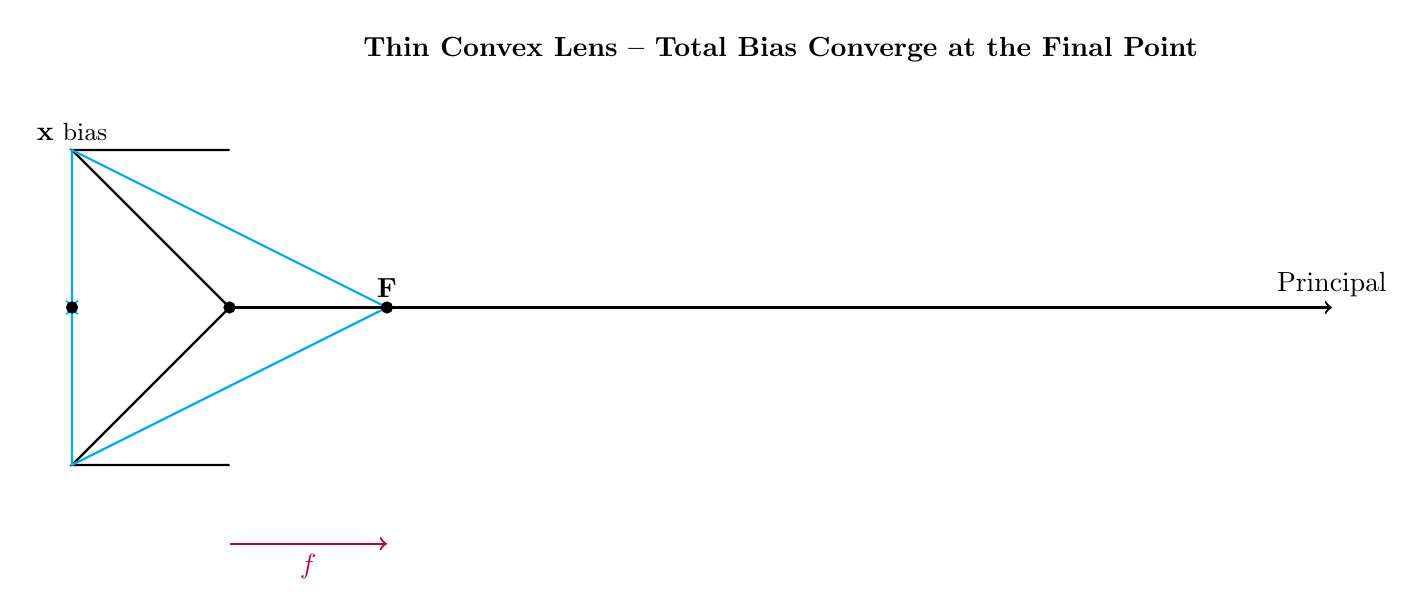
\begin{tikzpicture}
\draw[->,thick] (0,0) -- (14,0) node[above] {Principal};
\draw[fill] (0,0) circle (2pt);
\draw[thick] (0,0) -- (-2,2) -- (0,2);
\draw[thick] (0,0) -- (-2,-2) -- (0,-2);
\draw[->,thick,cyan] (2,0) -- (-2,2) -- (-2,0);
\draw[->,thick,cyan] (2,0) -- (-2,-2) -- (-2,0);
\draw[fill] (2,0) circle (2pt);
\draw[fill] (-2,0) circle (2pt);
\node[above] at (-2,2) {${\bf x}$ {\small bias}};
\node[above] at (2,0) {${\bf F}$};
\draw[->,thick,purple] (0,-3) -- (2,-3) node[midway,below] {$f$};
\node[above] at (7,3) {\textbf{Thin Convex Lens -- Total Bias Converge at the Final Point}};
\end{tikzpicture}

\end{document}